\section*{February}
\addcontentsline{toc}{section}{February}

\subsection*{02 02}
Managed to create conditional integrator. The problem is that you don't know how long the inegration might last so you can't allocate space for an array beforehand. There are basically a few solutions. You can append to numpy array, but every time you do that numpy has to reallocate the memory and its $\mathcal{O}(n^2)$ so super expensive. Another solution is to append to a regular array, which is $\mathcal{O}(1)$ and then you can allocate some memory beforehand, and if it exceedes the cap you can double itk, which is the solution I chose. First integrated a sample harmonic oscillator with a condition that if position reaches $x = x_{\rm end} = 0$ the integration stops.

\begin{center}
    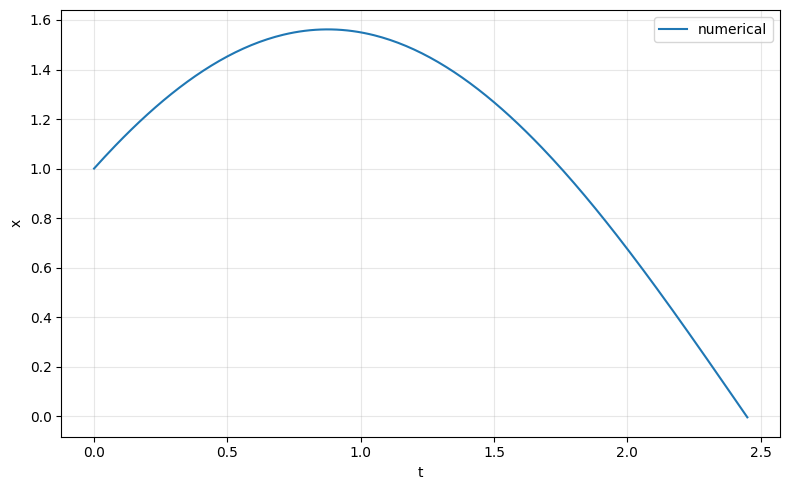
\includegraphics[width=250pt]{images/harmonic conditional.png}
\end{center}


Been learning how to derive geodesics in GR. In general we can use the arc length action:

\begin{equation*}
    S[x^{\mu}(\lambda)] = -mc \int ds = -mc \int d \lambda \sqrt{-g_{\mu \nu} \dot{x}^{\mu} \dot{x}^{\nu}},
\end{equation*}
where $\dot{x}^{\mu} \equiv \frac{d^{\mu}}{d \lambda}$ and $\lambda$ is a parameter along the worldline. To obtain the geodesics we extremise the action as usual. We can use a simpler and equivalent lagrangian

\begin{equation*}
    S^{\prime} (x(\lambda)) = \frac{1}{2} \int d \lambda \; g_{\mu \nu} (x) \dot{x}^{\mu} \dot{x}^{\nu}
\end{equation*}
Now we can apply Euler-Lagrange equations:

\begin{equation*}
    \frac{d}{d \lambda} \left( \frac{\partial L}{\partial \dot{x}^{\rho}} \right) - \frac{\partial L}{\partial x^{\rho}} = 0
\end{equation*}


\subsection*{02 03}
\begin{center}
    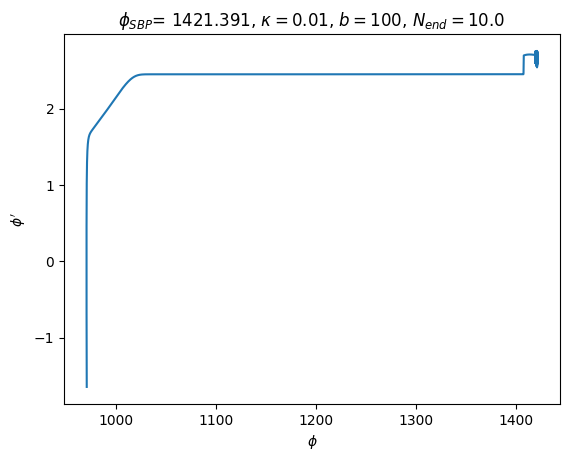
\includegraphics[width=250pt]{images/run1.png}
\end{center}

\subsection*{02 04}
Repeated the calculations for initial values for $\phi$ and $\phi^{\prime}$. Reminder, we're using $V(\phi) = V_0 \exp \left( - \kappa e^{\frac{\phi}{b}} \right)$ and we're taking $\mpl=1$. Start with the first slow-roll parameter $\epsilon$

\begin{equation*}
    \epsilon = \frac{1}{2} \left( \frac{V_{, \phi}}{V} \right) \quad \Rightarrow \quad \epsilon = \frac{1}{2} \left( \frac{\kappa}{b} \right)^2 \exp \left( \frac{2 \phi}{b} \right)
\end{equation*}
The inflation ends when $\epsilon = 1$ and this gives us $\phi_{\rm end}$

\begin{equation*}
    \phi_{\rm end} = \frac{b}{2} \ln \left[ \frac{2b^2}{\kappa} \right] \quad \Leftrightarrow \quad \exp \left[ \frac{\phi_{\rm end}}{b} \right] = \frac{\sqrt{2}b}{\kappa}
\end{equation*}

Using the slow-roll condition we can also obtain $\dot{\phi}_{\rm end}$ by evaluating the slow-roll equation at $\phi_{\rm end}$

\begin{equation*}
    3 H \dot{\phi} \approx - V_{, \phi} 
\end{equation*}
Note that we don't really care for $\dot{\phi}_{\rm end}$, at least for now. Using

\begin{equation*}
    H = \sqrt{\frac{V_0}{3}} \exp \left( -\sqrt{\frac{\alpha}{2}} \right) \quad \text{and} \quad V_{, \phi}(\phi) = V_0  \exp \left( - \kappa e^{\frac{\phi}{b}} \right) \left( \frac{-\kappa}{b} \right) e^{\frac{\phi}{b}}
\end{equation*}
then evaluating everything at $\phi_{\rm end}$ and plugging into the slow-roll equation

\begin{equation*}
    \dot{\phi}_{\rm end} = -\frac{V_{, \phi}}{3 H} = - \frac{V_0 \exp(-\sqrt{2}b)\sqrt{2}}{3\frac{\sqrt{V_0}}{\sqrt{3}} \exp \left( -\frac{b}{\sqrt{2}} \right)} = \sqrt{\frac{2}{3}} \sqrt{V_0} \exp \left( - \frac{\sqrt{2}}{2} \sqrt{2} \right) = \sqrt{\frac{2}{3} V_{\rm end}}
\end{equation*}

Next we solve the slow-roll equation and we can obtain the initial value $\phi_{i}$

\begin{align*}
    & \phi' \equiv \frac{d\phi}{dN} = - \frac{V_{,\phi}(\phi)}{V(\phi)} \quad
    \Rightarrow \quad \frac{d\phi}{dN} = \frac{\kappa}{b}\, \exp\!\left(\frac{\phi}{b}\right)\\
    \Rightarrow & \int_{\phi_i}^{\phi_f} \frac{b}{\kappa}\, \exp\!\left(-\frac{\phi}{b}\right)\, d\phi = \int_{N_i}^{N_f} dN = N_f - N_i.
\end{align*}
Note that we define $N \equiv \frac{\ln a}{\ln a(t_i)}$, then $N_i = 0$. Then

\begin{equation}\label{eq: subexpression for N}
    -\,\frac{b^{2}}{\kappa} \left[ \exp \! \left( -\frac{\phi_f}{b} \right) -\exp \! \left(-\frac{\phi_i}{b} \right) \right] = N_f
\end{equation}

At the end of inflation $\phi_f=\phi_{\rm end}$
\begin{equation}\label{eq: exp of phi_i}
    \frac{b^{2}}{\kappa} \left[ \frac{\sqrt{2}\, b}{\kappa} - \exp \! \left( -\frac{\phi_i}{b} \right) \right] = -\,N_{\text{end}} \quad \Rightarrow \quad \left( \frac{b}{\sqrt{2}} + N_{\text{end}} \right) = \frac{b^{2}}{\kappa} \, \exp\!\left(-\frac{\phi_i}{b}\right)
\end{equation}

\begin{equation*}
    \phi_i = - \, b \ln\!\left[ \frac{\kappa}{b^{2}} \left( \frac{b}{\sqrt{2}} + N_{\text{end}} \right) \right]
\end{equation*}

And now we similarly like before can compute the initial $\phi^{\prime}_i$ from the slow-roll equation

\begin{equation*}
    \phi^{\prime} = \frac{-V_{, \phi}}{3 H^2} \quad \Rightarrow \quad \phi^{\prime} = \frac{\kappa}{b} \exp(\frac{\phi}{b})
\end{equation*}

\begin{equation*}
    \phi^{\prime}_{i} = \frac{b}{\frac{b}{\sqrt{2}}+ N_{\rm end}}
\end{equation*}

And so we get the correct expressions compared to \href{https://journals.aps.org/prd/pdf/10.1103/PhysRevD.100.083530}{Mindaugas paper}. With a simple fix I was able to also produce some plots. First I varied $\kappa$ from 100 to 300

\begin{figure}[H]
    \centering
    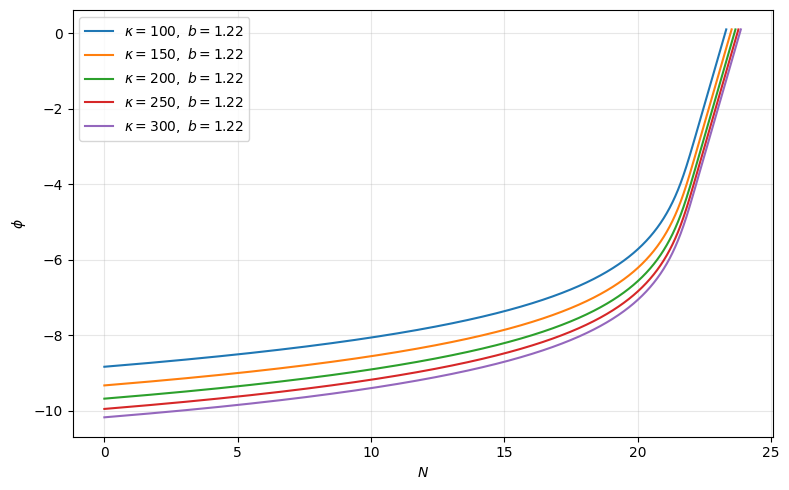
\includegraphics[width=0.48\textwidth]{images/phi_N_different_kappa.png}
    \hfill
    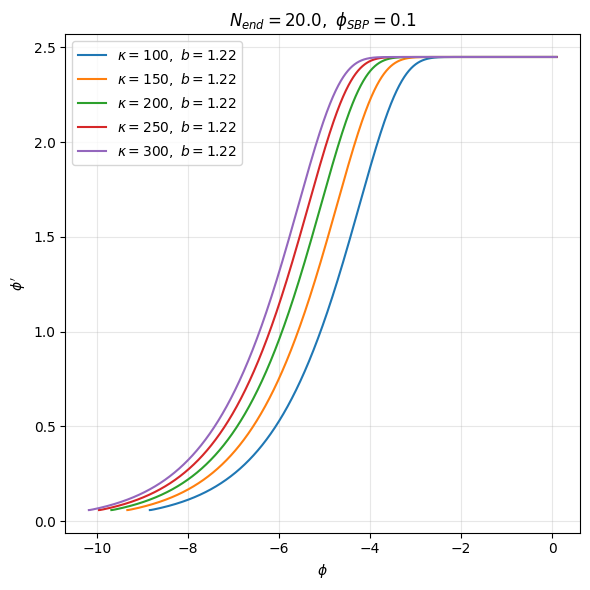
\includegraphics[width=0.48\textwidth]{images/phi_N_different_kappas.png}
    \caption{Varrying $\kappa$}
\end{figure}
Then I varied $b$ ($\alpha$ implicitly)

\begin{figure}[H]
    \centering
    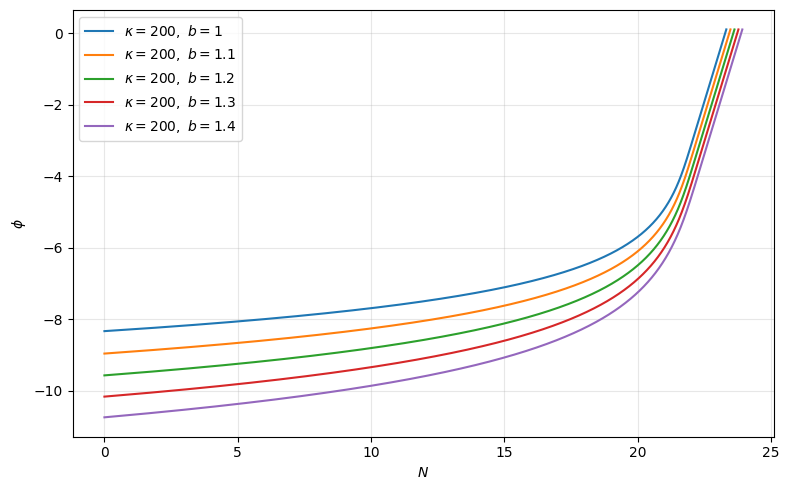
\includegraphics[width=0.48\textwidth]{images/phi_N_different_b.png}
    \hfill
    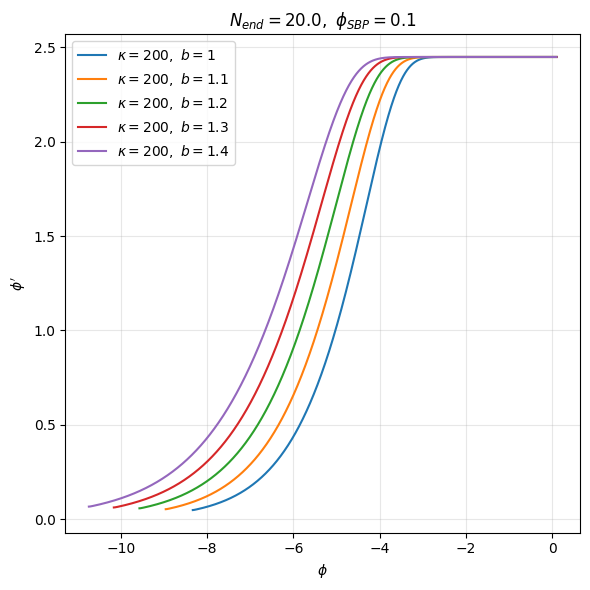
\includegraphics[width=0.48\textwidth]{images/phi_phi_prime_different_b.png}
    \caption{Varrying $\sqrt{\alpha}$}
\end{figure}
Tommorow I will probably try and compare the graphs with slowroll.


\subsection*{02 05}
Due to previous mistakes we redired the formula for $\phi(N)$ we start from (\ref{eq: subexpression for N}) then taking $N_f = N$ and exponential form of $\phi_i$ (\ref{eq: exp of phi_i}) to obtain

\begin{align*}
    & -\frac{b^2}{\kappa}\left[\exp\!\left(-\frac{\phi(N)}{b}\right)-\exp\!\left(-\frac{\phi_i}{b}\right)\right]=N \\
    \Rightarrow \quad & \exp\!\left(-\frac{\phi(N)}{b}\right)=-\frac{\kappa}{b^2}N+\exp\!\left(-\frac{\phi_i}{b}\right) \\
    \Rightarrow \quad & \phi(N)=-b\ln\!\left[\frac{\kappa}{b^2}\left(N_{\text{end}}-N\right)+\frac{\kappa}{b\sqrt{2}}\right]
\end{align*}
Notice that $N \lesssim N_{\rm end}$, due to the logarithm. Which just corresponds to the approximation working until the end of inflation, which makes sense. This now allows us to compare results

\begin{figure}[H]
    \centering
    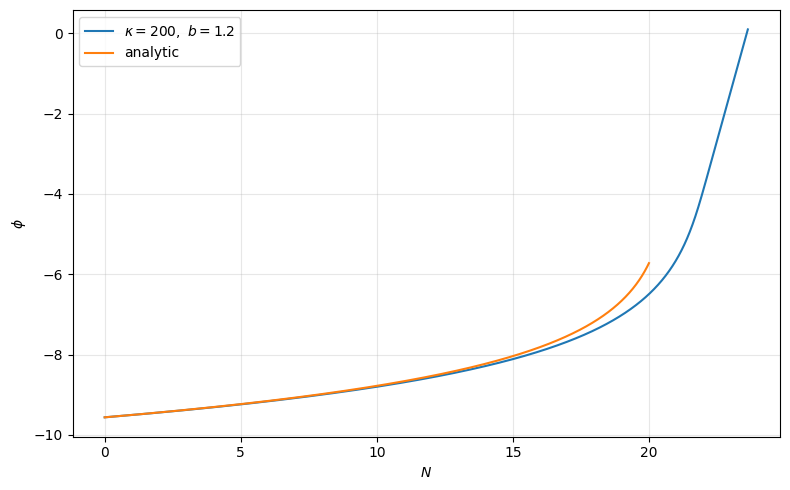
\includegraphics[width=0.48\textwidth]{images/analytic_slowroll_vs_numerical.png}
    \hfill
    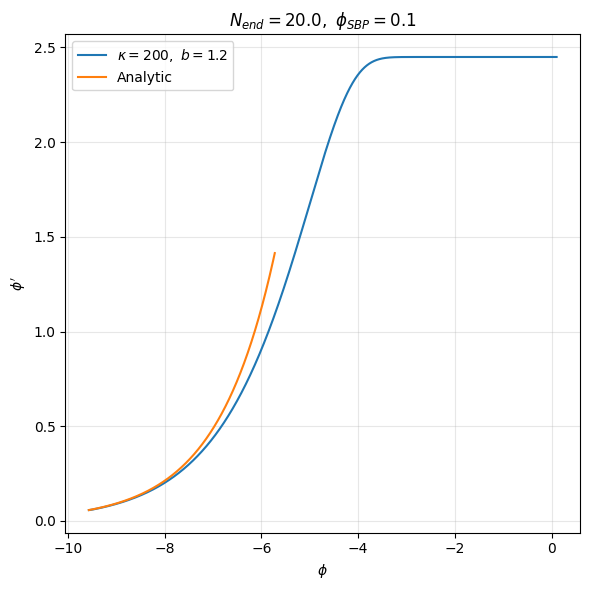
\includegraphics[width=0.48\textwidth]{images/analytic_SL_vs_numerical_phase_space.png}
    \caption{Numerical solutions vs Slow-roll analytic with $N_{\rm end} = 20.0$, $\kappa=200$, $b=\sqrt{\alpha}=1.2$, $\phi_{SBP} = 0.1$}
\end{figure}

Next, I should probably explore kination. In the kination limit the kinetic energy dominates so $\dot{\phi} \gg V_(\phi)$. Then Klein-Gordon equation takes the form

\begin{equation*}
    \ddot{\phi} + 3H \dot{\phi} \simeq 0
\end{equation*}
Again, changing integration variables from time to efolds

\begin{equation*}
    H^2 \phi^{\prime \prime} + \dot{H} \phi^{\prime} + 3 H^2 \phi^{\prime} = 0 \quad \Rightarrow \quad \phi^{\prime \prime} + \frac{\dot{H}}{H^2} \phi^{\prime} + 3 \phi^{\prime} = 0
\end{equation*}

But in the kination limit the Friedman equation reduces to $H^{2} = \frac{1}{3} \frac{1}{2} \dot{\phi}^2$. Hence

\begin{equation*}
    \frac{\dot{H}}{H^2} = \frac{-\frac{1}{2} \dot{\phi}^2}{\frac{1}{3} \frac{1}{2} \dot{\phi}^2} = -3.
\end{equation*}
Note, that this also gives the condition for kination in terms of $\epsilon$, i.e. $\epsilon = 3$. Combining these two results we're left with a trivial equation

\begin{equation*}
    \phi^{\prime \prime} - 3 \phi^{\prime} + 3 \phi^{\prime} = 0 \quad \Rightarrow \quad \phi^{\prime \prime} = 0.
\end{equation*}
Which has the following solution

\begin{equation*}
    \phi(N) = \phi^{\prime}_0 (N - N_f) + \phi_0
\end{equation*}
Here $\phi_0$ and $\phi^{\prime}_0$ are initial conditions for kination. In the paper Mindaugas writes that these correspond to the end of simulation (we stop simulation when $\phi$ reaches $\phi_{\rm SBP}$), so we can take $\phi_0$ from simulation and we can compute $\phi_{0}^{\prime}$ with $\epsilon=3$.

\begin{equation*}
    (\phi^{\prime})^2 = 2 \epsilon \quad \Rightarrow \quad \phi^{\prime} = \sqrt{6}
\end{equation*}
Then

\begin{equation*}
\phi(N) = \sqrt{6} \, (N - N_{\rm end}) + \phi_0
\end{equation*}
Where $N_{\rm end}$ is the efold number when the simulation ends. Then we are able to plot the results

\begin{figure}[H]
    \centering
    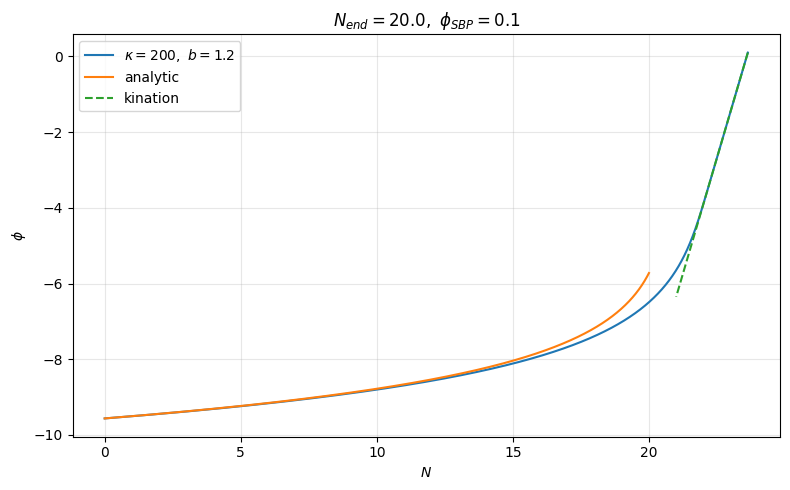
\includegraphics[width=0.48\textwidth]{images/kination_sr_phi_N.png}
    \hfill
    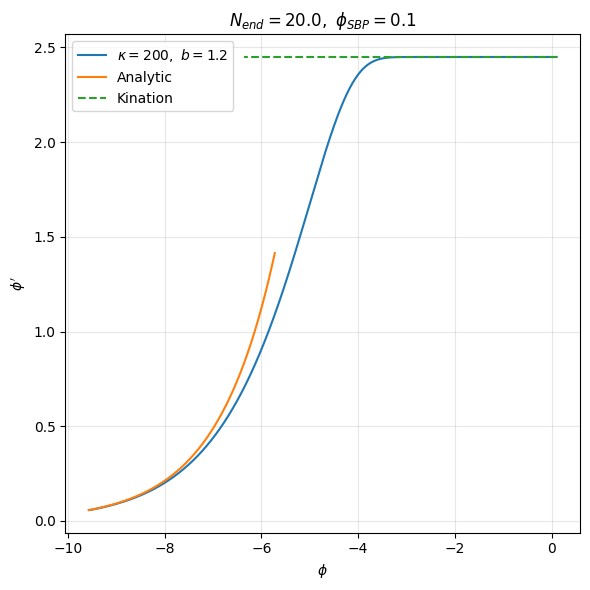
\includegraphics[width=0.48\textwidth]{images/kination_sr_phase.png}
    \caption{Numerical solutions vs Slow-roll analytic solution and kination}
\end{figure}


\subsection*{02 06}
Now that we have the homogeneous part done, we can start simulating $\chi$ values. Again we take a simplified version at first with vanishing self-coupling $\lambda=0$ and no evolution of $\theta$. So from Apostolos equations

\begin{equation*}
    \ddot{\tilde{\chi}}_{\bm{k}} + 3H \dot{\tilde{\chi}}_{\bm{k}} + \left[ \frac{k^2}{a^2} + g^2 (\phi - \phi_{\rm SBP})^2 \right] \tilde{\chi}_{\bm{k}} = 0
\end{equation*}
I can try again to change the integration variable to the number of efolds. There is a lot of interesting content in \href{https://arxiv.org/pdf/2112.11536}{the other paper also by Mindaugas}. 

Quitisential inflation is as I understand mostly defined by the shape of the potential: flat top to have slowroll, big gradient and then flat tail. Kination is a part of quitissential inflation and the fact that particles are not produced by the inflaton decay, but rather by non-perturbative effects. 

\subsection*{02 07}
Read part of the paper and got a slightly better understanding. One thing to note is that for initial conditions we take the Bunch-Davies vacuum state. 

\begin{equation}\label{eq: bunch davies initial conditions}
    \chi_{k, {\rm vac}} = \frac{a^{-1}}{\sqrt{2 \omega_k}} e^{-i \int^t \omega_k dt^{\prime}}
\end{equation}

What are these Bunch Davies initial conditions? First we define conformal time

\begin{equation*}
    d \eta = \frac{dt}{a(t)} \quad \text{then} \quad ds^2 = a(\eta)^2(-d \eta^2 + d \bm{x}^2),
\end{equation*}
where the conformal time defines the causal distance (or reach), s.t. $\Delta \eta$ gives the maximum causal distance light could travel, and like in Minkowski space, the causality structure is identical. Conformal time makes spacetime conformally flat. Next, we will investigate the dynamics of a scalar field, in FLRW. Consider the scalar field $\phi(\eta, \bm{x})$ and the above FLRW metric. Then the action (just the kinetic part) is given by

\begin{equation*}
    S = \int d^4x \sqrt{-g} \left[ - \frac{1}{2}g^{\mu \nu} \partial_{\mu} \phi \partial_{\nu} \phi \right].
\end{equation*}
Then from the metric we have $\sqrt{-g} = a^4(\eta)$, $g^{00}=-a^{-2}(\eta)$, $g^{ij} = \delta_{ij} a^{-2}(\eta)$. Inserting these into the metric we obtain

\begin{align*}
    S &= \int d^4x\, a^4(\eta)\left[-\frac{1}{2}\left(\frac{1}{a^2}\dot{\phi}^2 + \frac{1}{a^2(\eta)}(\nabla\phi)^2\right)\right]\\
    &= \int d^4x\, \frac{a^2}{2}\left(\phi'^2 - (\nabla\phi)^2\right).
\end{align*}
Varying the eqautions of motion with Euler-Lagrange equations (note that $\partial \mathcal{L}/ \partial \phi = 0$) we're left with:

\begin{equation*}
    \ddot{\phi} + 2 \frac{\dot{a}}{a} \dot{\phi} - \nabla^2 \phi = 0.
\end{equation*}
Next we expand $\phi$ in fourier space

\begin{equation*}
    \phi(\eta,\bm{x}) = \int \frac{d^3k}{(2\pi)^3}\,\phi_{\bm{k}}(\eta)\,e^{i\bm{k}\cdot\bm{x}} \quad \text{and} \quad \nabla^2 \phi(\eta,\bm{x}) = - \int \frac{d^3k}{(2\pi)^3}\,k^2\,\phi_{\bm{k}}(\eta)\,e^{i\bm{k}\cdot\bm{x}}.
\end{equation*}

\begin{align*}
    \int \frac{d^3k}{(2\pi)^3}\left[\ddot{\phi}_{\bm{k}}(\eta) + 2\frac{\dot{a}(\eta)}{a(\eta)}\dot{\phi}_{\bm{k}}(\eta) + k^2 \phi_{\bm{k}}(\eta)\right] e^{i\bm{k}\cdot\bm{x}} = 0\\
    \ddot{\phi}_{\bm{k}}(\eta) + 2\frac{\dot{a}(\eta)}{a(\eta)}\dot{\phi}_{\bm{k}}(\eta) + k^2 \phi_{\bm{k}}(\eta) = 0.
\end{align*}
Now we define a new variable $v(\eta, \bm{x}) = a(\eta) \phi(\eta, \bm{x})$, which in fourier space looks like $v_k(\eta) = a(\eta) \phi_k(\eta)$. Then we can express

\begin{align*}
    & \phi_k = \frac{v_k}{a} \\
    & \dot{\phi}_k = \frac{1}{a}\dot{v}_k - \frac{\dot{a}}{a^2}v_k \\
    & \ddot{\phi}_k = \frac{1}{a}\ddot{v}_k - \frac{2\dot{a}}{a^2}\dot{v}_k + \left(\frac{2\dot{a}^2}{a^3} - \frac{\ddot{a}}{a^2}\right)v_k
\end{align*}
Inserting everything, combining terms and cleaning up

\begin{equation*}
    \frac{\ddot{v}_k}{a} - \frac{2\dot{a}}{a^2}\dot{v}_k + \left(\frac{2\dot{a}^2}{a^3} - \frac{\ddot{a}}{a^2}\right)v_k + \frac{2\dot{a}}{a^2}\dot{v}_k - \frac{2\dot{a}^2}{a^3}v_k + k^2\frac{v_k}{a} = 0 \quad \Rightarrow \quad \frac{\ddot{v}_k}{a} - \left(k^2 - \frac{\ddot{a}}{a}\right)\frac{v_k}{a} = 0
\end{equation*}
Which gives the final result:

\begin{equation}\label{eq: similar to mukhanov sasaki}
    \ddot{v}_k + \left(k^2 - \frac{\ddot{a}}{a}\right)v_k = 0
\end{equation}

For small wavelengths we can disregard $\ddot{a}/a$ which yields

\begin{equation*}
    v_k(\eta) \xrightarrow[k\eta \to -\infty]{} \frac{1}{\sqrt{2k}}\,e^{-ik\eta} \quad \text{Equivalently} \quad \phi_k(\eta) \xrightarrow[k\eta \to -\infty]{} \frac{1}{a(\eta)\sqrt{2k}}\,e^{-ik\eta}
\end{equation*}
where the normalization comes from the Wronskian normalization, which I don't really understand... Either way, more generally the equation (\ref{eq: similar to mukhanov sasaki}) can be written

\begin{equation*}
    \ddot{v}_k + \omega_k^2(\eta)\,v_k = 0, \quad \text{where} \quad \omega_k^2(\eta) = k^2 + m_{\rm eff}^2(\eta)
\end{equation*}
There is an idea to rewrite the equations for $\chi$ to have something like these, but that's maybe for the future.

I basically want to simulate
\begin{equation*}
    \ddot{\chi}_{\bm{k}} + 3H \dot{\chi}_{\bm{k}} + \omega_{k} \chi_{\bm{k}} = 0
\end{equation*}
where $\omega_{k}^2 = \frac{k^2}{a^2} + g^2 (\phi - \phi_{\rm SBP})^2$. I am not sure which path to go, if I should change variables or not. I probably can try both. As for initial conditions, we need $\chi_k(t_0)$ and $\dot{\chi}_{k}(t_0)$ for the former we have equation (\ref{eq: bunch davies initial conditions}) where the exponential just gives a phase, so I think I can just have a trivial phase of $e^{0} = 1$ giving

\begin{equation}\label{eq: initial condition chi}
    \chi_k(t_0) = \frac{1}{a_0 \sqrt{2 \omega_{k,0}}}
\end{equation}
To get the initial values for $\dot{\chi}(t_0)$ we can just take a derivative. Note that for now I will ignore the chi energy density in $H$. Otherwise, I would need to recombine fourier modes and I will leave that for later. 

For now it makes sense to change the variables to e-folds as to have a simpler computation, since $\phi$.

Rewriting the equation in terms of e-fold number gives
\begin{equation*}
    H^2 \chi'' + H H' \chi' + 3 H^2  \chi' + \omega_k^2 \chi = 0 \quad \text{or} \quad \chi'' + \left( \frac{H'}{H} + 3 \right) \chi' + \frac{\omega_k^2}{H^2} \chi = 0
\end{equation*}


\subsection*{02 08}

In \href{https://arxiv.org/pdf/hep-ph/9704452}{\textit{Kofman paper}} I found a trick that can be easily derived, which sort of gets rid of the first derivative part. Suppose you have an equation of the form

\begin{equation*}
    \ddot{\chi} + 3\,\frac{\dot a}{a}\,\dot{\chi} + \omega^2 \chi = 0.
\end{equation*}
Then we can introduce a new variable $\chi = a^n X$ and the goal is to find $n$ such that the first derivative terms vanish and we're left if a harmonic-oscillator type of equation. The derivative terms give us

\begin{align*}
    \dot{\chi} &= n a^{n-1}\dot{a} \, X + a^{n}\dot{X} \\
    \ddot{\chi} &= n(n-1)a^{n-2}\dot{a}^{2} X + n a^{n-1}\ddot{a} \, X + n a^{n-1}\dot{a}\,\dot{\chi} + n a^{n-1}\dot{a}\,\dot{X} + a^{n}\ddot{X}
\end{align*}

Inserting into the equation and only looking at the first derivative terms we have

\begin{equation*}
    \left[ 2n a^{n-1} \dot{a} + a^n 3 \frac{\dot{a}}{a} \right] \dot{X}
\end{equation*}
We want these terms to vanish, so we set the coefficient to 0 and get $n=-\frac{3}{2}$. Then we can recombine the remaining terms, using the new value of $n$. Giving us just

\begin{equation}\label{eq: X harmonic equation}
\ddot{X} + \left[ \omega^2 - \frac{3}{2}\frac{\ddot a}{a} - \frac{3}{4}\frac{\dot a^2}{a^2} \right] X = 0
\end{equation}
and by definition of the Hubble parameter $H = \frac{\dot a}{a}$ and $\dot H = \frac{\ddot a}{a} - \frac{\dot a^2}{a^2}$ we can rewrite these equations even more concisely. This is just an illustrative example, maybe I can try and rewrite the equations of motion like that, but using number of efolds as my integration variable.

I tried that, but it doesn't work due to the additional $+3$ term. For now I will integrate wrt efold number, forget about optimisation and will discuss these things with Mindaugas. It can also be seen that it doesn't work from the above equation, if you were top introduce integration wrt efold number then the second derivative would give you first derivative.


\subsection*{02 09}
I want to simulate these equations

\begin{align*}
    \ddot{\phi} + 3H \dot{\phi} + V_{, \phi} = 0, \\
    \ddot{\chi}_k + 3H \dot{\chi} + \omega^2_k \chi = 0,
\end{align*}
which in conformal time $\eta$ take the form

\begin{align}\label{eq: conformal time eom}
    \phi'' + 2 \mathcal{H} \phi' + a^2 V_{, \phi} = 0,\\
    \chi'' + 2 \mathcal{H} \chi'_k + a^2 \omega_k^2 \chi_k = 0.
\end{align}
Here $\mathcal{H}$ is the hubble parameter in conformal time s.t. $\mathcal{H} = \frac{a'}{a}$. Then making substitutions $\Phi = a \phi$ and $X_k = a \chi_k$ we obtain equations, which are similar to Mukhanov equations

\begin{align}\label{eq: conformal time mukhanoc}
    \Phi'' + \left( a^2 V_{, \phi \phi} - \frac{a''}{a} \right) \Phi = 0, \\
    X_k'' + \left( a^2 \omega_k^2 - \frac{a''}{a} \right) X_k = 0.
\end{align}
Don't know if there is much use out of these equations, but here they are.

Let's return to initla conditions for $\chi$ and $\dot{\chi}$. We already know the initial condition for $\chi$ that is equation (\ref{eq: initial condition chi}). For $\dot{\chi}_k$ we first find the derivative and then again insert $t_0$.

\begin{equation*}
    \dot{\chi}_k = \frac{d}{dt} \left( \frac{a^{-1}}{\sqrt{2 \omega_k}} \right) \exp \left( -i \int^t \omega_k dt' \right) + \frac{a^{-1}}{\sqrt{2 \omega_k}} \frac{d}{dt} \left( \exp \left( -i \int^t \omega_k dt' \right) \right)
\end{equation*}


\subsection*{02 10}
How do we determine the range for $k$ modes? For large $k$, (UV bound) $\frac{k^2}{a^2} \gg H^2$ and so the dynamics becode that of a free wave $\chi \sim e^{\pm i k t}$. Similarly, for small $k$ we have $\frac{k^2}{a^2} \ll H^2$, which entails that $\omega^2_k$ becomes unimportant. But note that the bounds move with time $\frac{k}{aH} \propto e^{-N}$ and logarithmic spacing is required.

\begin{equation*}
    k_{\rm min} = a(t_{\rm start}) H(t_{t_{start}}), \qquad k_{\rm min} = \zeta a(t_{\rm SBP}) H(t_{t_{SBP}})
\end{equation*}
with $\zeta \approx 10-100$.

\subsection*{02 11}
It does seem like at least for now it is the most useful to do the computation for homogeneous $\phi$ field wrt the number of efolds. The problem that I encountered was converting from $N$ to $t$. We use the simple relation

\begin{equation*}
    \dot{\phi} = H \phi' \quad \Rightarrow \quad \frac{d \phi}{d t} = H \frac{d \phi}{d N} \quad \Rightarrow \quad \int dt = \int \frac{1}{H} dN
\end{equation*}
and we determine $H$ via Friedman equation in $N$

\begin{equation*}
    H^2 = \frac{V(\phi)}{3 - \frac{1}{2} \phi'^2}.
\end{equation*}
In code the integration is made with the trapezoid rule.


\subsection*{02 12}
Wrote the code for converting $N$ to $t$ and plotted the results

\begin{figure}[h!]
    \centering
    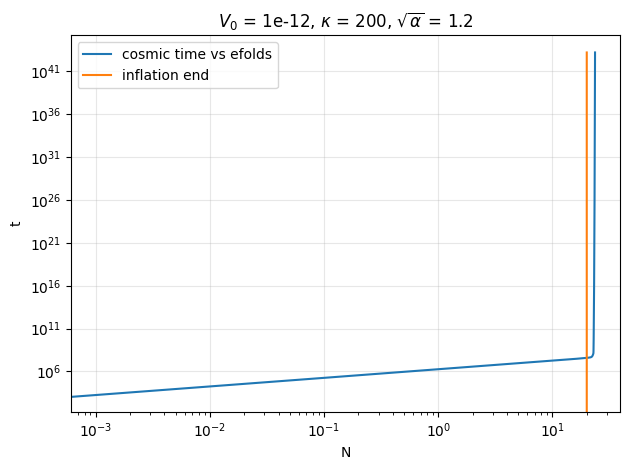
\includegraphics[width=0.5\textwidth]{images/N_t_graph.png}
    \caption{The orange vertical line marks $N=20$, i.e. the end of inflation. Both $N$ and $t$ are in $\log$ scales.}
\end{figure}

To get a better view of the $N(t)$ after the inflation it's usefull to "zoom in" and "turn off" log scales. Note that to find the intersection we just check when the difference of $N$ and $N_{\rm end} = 20$ changes sign.

\begin{figure}[h!]
    \centering
    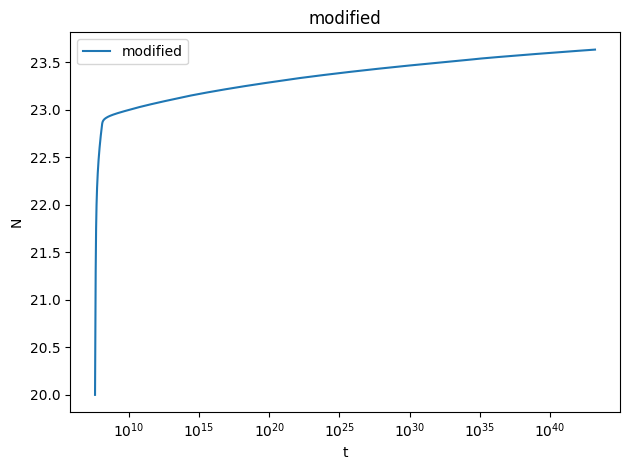
\includegraphics[width=0.5\textwidth]{images/N_to_t_mod.png}
    \caption{$t$ is on log scale, while $N$ is linear}
\end{figure}

For missing values one can interpolate.

Initial conditions yet again. One needs to be careful when looking at the initial conditions from Mindaugas papaer, since our $\omega_k^2 = \frac{k^2}{a^2} + \dots$ i.e. we use additional division by $a^2$. To start, consider the WKB approximation. As a reminder, consider the differential equation

\begin{equation*}
    y''(x) + Q(x) y(x) = 0 \quad \text{or} \quad y''(x) + \omega^2(x) y(x) = 0
\end{equation*}
where $\omega(x) = \sqrt{Q(x)}$. WKB approximation is built on the assumption that $\omega(x)$ varies slowly. To put that mathematically, if $\omega(x) = {\rm const}$ then the solution would be $y(x) \sim e^{ \pm i \omega x}$ with a natural wavelength $\lambda(x) = \frac{2 \pi}{\omega(x)}$, meaning $\Delta x \sim \frac{1}{\omega}$. And from Taylor series we have $\Delta \omega \simeq \omega'(x) \Delta x$, thus

\begin{equation*}
    \Delta x \sim \frac{1}{\omega} \quad \Rightarrow \quad \Delta \omega \sim \frac{\omega'}{\omega}    
\end{equation*}
But we want for $\omega$ to change very little during one oscillation, meaning $\frac{\Delta \omega}{\omega} \ll 1$. Hence the condition $ \left| \frac{\omega'}{\omega^2} \right| \ll 1$. To use WKB approximation we use the ansatz $y=A(x) e^{iS(x)}$, then

\begin{align*}
    y' &= (A'+iAS')e^{iS}\\
    y'' &= (A'' + 2iA'S' + iAS'' - AS'^2) e^{iS}
\end{align*}
then
\begin{equation*}
    A'' + 2iA'S' + iAS'' - AS'^2 + \omega^2 A = 0
\end{equation*}
Let's now take a step back. Again, is $\omega$ was constant the exponential factor would be $\omega_k x$, which in all actuallity is the integral, so we have $S' \sim \omega$ (writting the derivative so that we can easily see the $\omega$), then $S'' \sim \omega'$. Now we can investigate the asymptotic behaviour. Split the equation into real and imaginary parts. The imaginary part gives:

\begin{equation*}
    2A'S' + AS'' = 0 \quad \Rightarrow \quad \frac{A'}{A} = -\frac{S''}{2 S'} \quad \Rightarrow \quad \frac{A'}{A} \sim \frac{\omega'}{\omega}.
\end{equation*}
Likewise, the real part gives

\begin{equation*}
    A'' - AS'^2 + \omega^2 A = 0 \quad \Rightarrow \quad A'' = (S'^2 - \omega^2) A \quad \Rightarrow \quad A'' \sim (\omega^2 - \omega^2) A = 0
\end{equation*}
which means that $A''$ is negligable. This now simplifies the main equation to

\begin{equation*}
    -AS'^2 + \omega^2 A + 2iA' S' + iAS'' = 0
\end{equation*}
After seperating real and imaginary parts we obtain:

\begin{equation*}
    -AS'^2 + \omega^2 A = 0 \quad \text{and} \quad 2 A' S' + A S'' = 0 
\end{equation*}
which yield the solutions $S(x) = \pm \int^x \omega(x') dx'$ and $A(x) = \frac{C}{\sqrt{\omega(x)}}$. Hence the WKB solution is

\begin{equation}\label{eq: WKB mathematical solution}
    y(x) \simeq \frac{C}{\sqrt{\omega_k}} \exp(-i \int^t \omega_k(x') dx')
\end{equation}
Next we investigate the normalization with the Wronskian


\subsection*{02 13}

Consider some complex KG field $\hat{\phi}(t, \bm{x})$

\begin{equation*}
    \hat{\phi}(t,\mathbf{x}) = \int \frac{d^3 \mathbf{k}}{(2\pi)^3}
    \left( \phi_{\mathbf{k}}(t)\,\hat{a}_{\mathbf{k}}\, e^{i \mathbf{k}\cdot \mathbf{x}} + \phi_{\mathbf{k}}^*(t)\,\hat{a}_{\mathbf{k}}^\dagger\, e^{-i \mathbf{k}\cdot \mathbf{x}}
    \right)
\end{equation*}
and conjugate momenta $\hat{\pi} (t. \bm{x}) = \dot{\hat{\phi}}(t,\bm{x})$
\begin{equation*}
    \hat{\pi}(t,\mathbf{x}) = \int \frac{d^3 \mathbf{q}}{(2\pi)^3}
    \left( \phi'_{\mathbf{q}}(t)\,\hat{a}_{\mathbf{q}}\, e^{i \mathbf{q}\cdot \mathbf{x}} + \phi_{\mathbf{q}}^{*\prime}(t)\,\hat{a}_{\mathbf{q}}^\dagger\, e^{-i \mathbf{q}\cdot \mathbf{x}}
    \right).
\end{equation*}
Thus from the canonical commutation relations $[\hat{\phi}(t, \bm{x}), \hat{\pi}(t, \bm{y})] = i \delta^{3}(\bm{x} - \bm{y})$ we have
\begin{align*}
[\hat{\phi}(t,\mathbf{x}), \hat{\pi}(t,\mathbf{y})]
&=
\int \frac{d^3 \mathbf{k}}{(2\pi)^3}
\int \frac{d^3 \mathbf{q}}{(2\pi)^3}
\Big(
\phi_{\mathbf{k}}(t)\,\phi'_{\mathbf{q}}(t)\,
[\hat{a}_{\mathbf{k}}, \hat{a}_{\mathbf{q}}]\,
e^{i(\mathbf{k}\cdot\mathbf{x} + \mathbf{q}\cdot\mathbf{y})}\\
&\quad
+\, \phi_{\mathbf{k}}(t)\,\phi_{\mathbf{q}}^{*\prime}(t)\,
[\hat{a}_{\mathbf{k}}, \hat{a}_{\mathbf{q}}^\dagger]\,
e^{i(\mathbf{k}\cdot\mathbf{x} - \mathbf{q}\cdot\mathbf{y})}\\
&\quad
+\, \phi_{\mathbf{k}}^*(t)\,\phi'_{\mathbf{q}}(t)\,
[\hat{a}_{\mathbf{k}}^\dagger, \hat{a}_{\mathbf{q}}]\,
e^{i(-\mathbf{k}\cdot\mathbf{x} + \mathbf{q}\cdot\mathbf{y})}\\
&\quad
+\, \phi_{\mathbf{k}}^*(t)\,\phi_{\mathbf{q}}^{*\prime}(t)\,
[\hat{a}_{\mathbf{k}}^\dagger, \hat{a}_{\mathbf{q}}^\dagger]\,
e^{i(-\mathbf{k}\cdot\mathbf{x} - \mathbf{q}\cdot\mathbf{y})}
\Big).
\end{align*}
but $[\hat{a}_{\mathbf{k}}, \hat{a}_{\mathbf{q}}] = [\hat{a}_{\mathbf{k}}^\dagger, \hat{a}_{\mathbf{q}}^\dagger] = 0$ and $[\hat{a}_{\mathbf{k}}, \hat{a}_{\mathbf{q}}^\dagger] = -[\hat{a}_{\mathbf{k}}^\dagger, \hat{a}_{\mathbf{q}}] = (2 \pi)^3 \delta^3(\bm{x} - \bm{y})$. Hence

\begin{align*}
    &=\int \frac{d^3 \mathbf{k}}{(2\pi)^3} \int \frac{d^3 \mathbf{q}}{(2\pi)^3}
    \Big( \phi_{\mathbf{k}}(t)\,\phi_{\mathbf{q}}^{*\prime}(t)\,
    (2\pi)^3 \delta^{(3)}(\mathbf{k}-\mathbf{q})\,
    e^{i(\mathbf{k}\cdot\mathbf{x} - \mathbf{q}\cdot\mathbf{y})} \\
    &\qquad
    -\, \phi_{\mathbf{k}}^*(t)\,\phi'_{\mathbf{q}}(t)\,
    (2\pi)^3 \delta^{(3)}(\mathbf{k}-\mathbf{q})\,
    e^{i(-\mathbf{k}\cdot\mathbf{x} + \mathbf{q}\cdot\mathbf{y})} \Big) \\
    &= \int \frac{d^3 \mathbf{k}}{(2\pi)^3}
    \left( \phi_{\mathbf{k}}(t)\,\phi_{\mathbf{k}}^{*\prime}(t)\,
    e^{i\mathbf{k}\cdot(\mathbf{x}-\mathbf{y})} - \phi_{\mathbf{k}}^*(t)\,\phi'_{\mathbf{k}}(t)\, e^{i\mathbf{k}\cdot(\mathbf{y}-\mathbf{x})}
    \right). \\
    &=\left( \phi_{\mathbf{k}}(t)\,\phi_{\mathbf{k}}^{*\prime}(t) - \phi_{\mathbf{k}}^*(t)\,\phi'_{\mathbf{k}}(t) \right) \delta^{(3)}(\mathbf{x} - \mathbf{y}).
\end{align*}
Them comparing to the RHS of canonical commutation relation we have
\begin{equation}\label{eq: wronskian}
    \phi_{\mathbf{k}}\,\phi_{\mathbf{k}}^{*\prime} - \phi_{\mathbf{k}}^*\,\phi'_{\mathbf{k}} = i
\end{equation}
Which is defined as the Wronskian $W$. 

We now can combine everything. There are two ways of doing this, i.e. how we define the vacuum. We either define it from conformal time or from cosmic time. First, let's take a look at the latter

Consider the equation (\ref{eq: X harmonic equation}), and rewrite it as

\begin{equation*}
    \ddot{X} + \Omega^2_k X = 0 \quad \text{with} \quad X = a^{3/2} \chi
\end{equation*}
where $\Omega^2_k(t) = \omega^2_k - \frac{3}{2} \frac{\ddot{a}}{a} - \frac{9}{4} \frac{\dot{a}^2}{a^2} = \omega^2_k - \frac{3}{2} \dot{H} - \frac{9}{4} H^2$. Then using WKB approximation we know the solution must look like equation (\ref{eq: WKB mathematical solution}). Hence

\begin{equation*}
    X_k = \frac{C}{\sqrt{2\Omega_k(t)}} \exp\left(-i \int^{t} \Omega_k(t')\,dt'\right) \quad \text{and} \quad X_k^* = \frac{C}{\sqrt{2\Omega_k(t)}} \exp\left(i \int^{t} \Omega_k(t')\,dt'\right)
\end{equation*}

\begin{align*}
\dot{X}_k
&= -\frac{1}{2}\frac{C\,\dot{\Omega}}{\sqrt{2\Omega}\,\sqrt{\Omega}} \exp\!\left(-i\int^{t}\Omega(t')\,dt'\right)
- i\,\frac{C}{\sqrt{2\Omega_k(t)}} \exp\!\left(-i\int^{t}\Omega(t')\,dt'\right)\Omega(t) \\[6pt]
\Rightarrow  \dot{X}_k &= -\frac{1}{2}\frac{\dot{\Omega}}{\Omega}X_k - i\Omega X_k
\quad \text{and} \quad
\dot{X}_k^{*} = -\frac{1}{2}\frac{\dot{\Omega}}{\Omega}X_k^{*} + i\Omega X_k^{*}
\end{align*}
Then note that $X_u X_u^{*} = \frac{C^2}{2\Omega_u(t)}$ and by using the Wronskian (\ref{eq: wronskian}) we obtain

\begin{equation*}
    X_k \dot{X}_k^{*} - X_k^{*} \dot{X}_k = i \quad \Rightarrow \quad 2i\, X_k X_k^{*} \Omega = i \quad \Rightarrow \quad 2 \frac{C^2}{2\Omega(t)} \Omega = 1 \quad \Rightarrow \quad C = \pm 1
\end{equation*}
We only take the positive modes. Hence we obtain the vacuum solution

\begin{equation*}
    \chi_k = \frac{a^{-3/2}}{\sqrt{2\Omega_k}} \exp\left(-i \int^{t} \Omega_k(t')\, dt' \right) \quad \text{where} \quad \Omega^2_k(t) = \omega^2_k - \frac{3}{2} \dot{H} - \frac{9}{4} H^2
\end{equation*}

There is an alternative way of computing the vacuum, namely by first converting to conformal time and only then following the same procedure. It is often considered a good practice to quantize everything in conformal time, since it maintains causal structure. The equations of motion would then be equations (\ref{eq: conformal time eom}) and after substitution $X = a \chi$ we obtain Mukhanov type of equations (\ref{eq: conformal time mukhanoc}). This now allows us to use the WKB approximation again. 

\begin{equation*}
    X''_k + \Omega^2_k(\eta) X_k = 0 \quad \text{where} \quad \Omega^2_k(\eta) = a^2 \omega^2_k - \frac{a''}{a}
\end{equation*}
After a similar procedure as before we obtain

\begin{equation*}
    \chi_k = \frac{a^{-1}}{\sqrt{2 \Omega_k}} \exp(-i \int^\eta \Omega_k(\eta')d \eta')
\end{equation*}


\subsection*{02 15}

The final step is to convert this expression to cosmic time, so that we could compare the vacuum states. First, remember that conformal time is defined as $d \eta = \frac{d t}{a}$, so

\begin{equation*}
    a' = \frac{d}{d \eta} = \frac{dt}{d \eta} \frac{d}{dt} (a) = a \dot{a} \quad \text{and} \quad a'' = a \frac{d}{dt} (a \dot{a}) = a(\dot{a}^2 + a \ddot{a})
\end{equation*}
then

\begin{equation*}
    \Omega_k^2(\eta) = a^2 \omega^2_k - \frac{a''}{a} = a^2 \omega^2_k - (\dot{a}^2 + a \ddot{a}) = a^2 (\omega^2_k - \dot{H} - 2 H^2)
\end{equation*}
For convenience define $\Omega_k^2 = a^2 \tilde{\Omega}_k^2$, so $\tilde{\Omega}_k^2 = \omega^2_k - \dot{H} - 2 H^2$. Then the exponential part becomes

\begin{equation*}
    \exp \left( \int^{\eta} \Omega_k (\eta ') d \eta' \right) = \exp( \int^\eta \Omega_k(t') \frac{d \eta'}{a}) = \exp(\int^t \tilde{\Omega}_k d t')
\end{equation*}
Combining everything we obtain

\begin{equation*}
    \chi_k = \frac{a^{-3/2}}{\sqrt{2 \tilde{\Omega}_k}} \exp \left( \int^t \tilde{\Omega}_k dt' \right) \quad \text{where} \quad \tilde{\Omega}_k^2 = \omega^2_k - \dot{H} - 2H^2
\end{equation*}
This is different from the previous result. Since we just want initial conditions for the numerical simulations at $t=0$ we have $a=1$ and a lot of stuff simplifies, leaving

\begin{align*}
    &\text{Cosmic Time:} &\chi_k = \frac{1}{\sqrt{2 \Omega_k}} \quad \text{with} \quad &\Omega_k^2 = \omega^2_k - \frac{3}{2}\dot{H} - \frac{9}{4} H^2\\
    &\text{Conformal Time:} &\chi_k = \frac{1}{\sqrt{2 \tilde{\Omega}_k}} \quad \text{with} \quad &\tilde{\Omega}_k^2  = \omega^2_k - \dot{H} - H^2
\end{align*}
and for $\dot{\chi}$

\begin{align*}
    &\text{Cosmic Time:} &\dot{\chi}_k = \left( -\frac{3}{2}H -\frac{1}{2}\frac{\dot{\Omega}_k}{\Omega_k} - i\,\Omega_k \right)\chi_k \quad \text{with} \quad \dot{\Omega}_k = \frac{1}{2\Omega_k} \left[ \dot{\omega}^2_k - \frac{3}{2}\ddot{H} -\frac{9}{2} H \dot{H} \right]
    \\
    &\text{Conformal Time:} &\dot{\chi}_k = \left( -\frac{3}{2}H -\frac{1}{2}\frac{\dot{\tilde{\Omega}}_k}{\tilde{\Omega}_k} - i\,\tilde{\Omega}_k \right)\chi_k \quad \text{with} \quad \dot{\tilde{\Omega}}_k = \frac{1}{2\tilde{\Omega}_k} \left[ \dot{\omega}^2_k -\ddot{H} -2H\dot{H} \right]
\end{align*}
with $\dot{\omega}^2_k = -2H\frac{k^2}{a^2} +2g^2(\phi-\phi_{\mathrm{SBP}})\dot{\phi}$.

After simulating everything we obtain a preliminary plot

\begin{figure*}
    \centering
    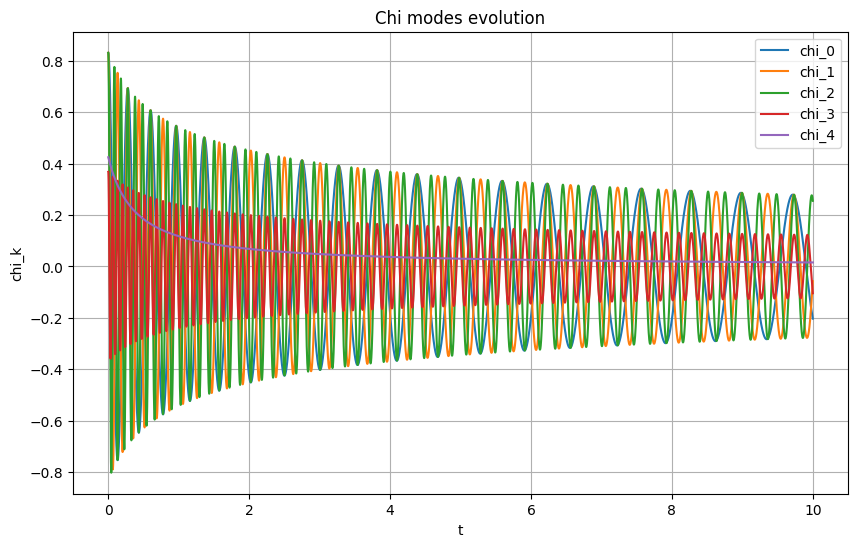
\includegraphics[width=0.5 \textwidth]{images/chi_first.png}
\end{figure*}